% !TEX root = ../main.tex
%
\section{Introduction}
\label{sec:introduction}

Research on conversational moderation/facilitation techniques\footnote{Distinct from “content moderation”, which involves flagging and removing content. The terms “facilitation” and “conversational moderation” are otherwise equivalent \cite{argyle2023, korre2025evaluation, falk-etal-2021-predicting}. We use the terms interchangeably in this paper.} is crucial for adapting to ever-changing and demanding online environments. Relevant work traditionally focused on isolating and removing content \cite{seering_self_moderation, cresci_pesonalized_interventions}, whereas the current social media environment demands moderation systems to adequately explain their actions and prevent problematic behaviors before they surface \cite{cho-etal-2024-language, seering_self_moderation, cresci_pesonalized_interventions, make_reddit_great} as well as handle community tasks \cite{kim_et_al_chatbot, seering_self_moderation}.

\begin{figure}[hbt!]
	\centering
	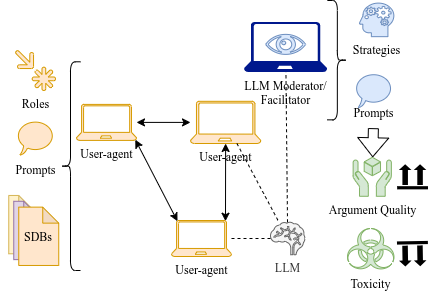
\includegraphics[width=\columnwidth]{research_goal.png}
	\caption{The \ac{LLM} user-agents conduct a discussion, while the \ac{LLM} moderator monitors and attempts to increase its quality. We need to design prompts and configurations for both.}
	\label{fig::goals}
\end{figure}

A major challenge in pivoting research to current demands lies in the substantial costs required both in researching and moderating discussions, due to human participation \cite{rossi_2024}. Many social media platforms overcome this by outsourcing moderation to volunteers or their own users \cite{Matias2019TheCL, schaffner_community_guidelines}, while others turn to content moderation using traditional \ac{ML} models, which are not enough in practice \cite{horta_automated_moderation, schaffner_community_guidelines}. \acfp{LLM} have been hypothesized to be capable of conversational moderation and facilitation tasks \cite{small-polis-llm, korre2025evaluation}. 

While studies exist for simulating user interactions in social media \cite{park_simulacra, mou_2024, tornberg_2023, y_social, balog_2024}, and for using synthetic facilitators \cite{kim_et_al_chatbot, cho-etal-2024-language}, none so far have combined the two approaches. We posit that synthetic simulations can be a cheap and easy way to prototype the development of inherently unstable and unpredictable (w.r.t. prompting) \cite{atil_2025, rossi_2024} \ac{LLM} moderators. Our work thus asks the following two questions: (1) Can we produce high-quality synthetic data by crafting an appropriate environment for simulations? (2) Can we boost the effectiveness of \ac{LLM} moderators (in synthetic discussions) by using prompts aligned with current Social Science research?

We propose a simple and generalizable approach using \ac{LLM}-driven synthetic experiments for online moderation research, enabling fast and inexpensive model “debugging” and parameter testing (e.g.,  \ac{LLM} moderator prompts, instructions) without human involvement (Section~\ref{sec:methodology}) (Fig.~\ref{fig::goals}). An ablation study (Section~\ref{ssec:results:ablation}) demonstrates that each step of our methodology meaningfully contributes to generating high-quality synthetic data, as well as examining the output of various \acp{LLM}. Using this methodology, we examine four \ac{LLM} moderation strategies based on current Social Science facilitation research (Section~\ref{sec:experimental})
%: \ac{LLM} alignment guidelines \cite{collective_constitution}, prompts based on human facilitation guidelines \cite{Cornell_eRulemaking2017, dimitra-book} and our own prompt based on \ac{RL} (although we do not perform \ac{RL} in this paper). We 
and compare them with two baselines via \ac{LLM} annotator-agents.

Our analysis reveals two key findings (Section \ref{sec:results}): (1) the presence of \ac{LLM} moderators exhibited a positive and statistically significant influence on the quality of synthetic discussions, and (2) current moderation strategies are often not enough to meaningfully outperform simple baselines. %However, besides helping in understanding the effect of prompts to \ac{LLM} moderators, the synthetic data presented in this paper can also be used to finetune them.
Furthermore, we release \syndisco an open-source Python framework for generating and evaluating synthetic discussions, alongside \vmd\datasetlink a large, publicly available dataset comprising the evaluated discussions (Section~\ref{sec:data-soft}). %Finally, we outline the limitations (Section~\ref{sec:limitations}) and ethical considerations (Section~\ref{sec:ethical}) of our work. 
We use open-source \acp{LLM} and include all relevant configurations in order to make our study as reproducible as possible (see Appendix \ref{ssec:appendix:annotation}, \ref{ssec:appendix:prompts}).